\documentclass[sigconf]{acmart}

\AtBeginDocument{%
  \providecommand\BibTeX{{Bib\TeX}}}

\copyrightyear{2023}
\acmYear{2023}
\setcopyright{rightsretained}
\acmConference[AIM 2023]{Proceedings of the UNamur
Symposium on Advanced Interaction Methods}{December 14,
2023}{Namur, Belgium}
\acmBooktitle{Proceedings of the UNamur
Symposium on Advanced Interaction Methods (AIM 2023 Proceedings), December 14, 2023,
Namur, Belgium}
\acmDOI{00.0000/0000000.0000000}
\acmISBN{000-0-0000-0000-0/00/00}

\usepackage{xspace}
\newcommand{\ie}{\textit{i.e.},\xspace}
\newcommand{\eg}{\textit{e.g.},\xspace}
\newcommand{\vs}{\textit{vs.}\xspace}
\newcommand{\etal}{\textit{et al.}\xspace}

\begin{document}

%%
%% Title
\title[SoundWay: BLE-Based Augmented Navigation]{SoundWay: A BLE Multi-Advertising System with Voice Interaction and Mobile Feedback for Indoor Orientation Assistance}

%%
%% Authors
\author{Esteban BARRACHO}
\email{esteban.barracho@student.unamur.be}

\author{Anas DAMLAKHI}
\email{anas.damlakhi@student.unamur.be}

\author{Jonathan KONDOLI NKEBI}
\email{jonathan.kondolinbk@student.unamur.be}

\author{Arthur SMOOS}
\email{arthur.smoos@student.unamur.be}

\author{Bénédicte TUTEKA MUKUTA}
\email{benedicte.tutekamukuta@student.unamur.be}

\affiliation{
  \institution{University of Namur, Faculty of Computer Science}
  \streetaddress{Rue Grandgagnage, 21}
  \city{Namur}
  \postcode{B-5000}
  \country{Belgium}
}

\renewcommand{\shortauthors}{Barracho et al.}

%%
%% Teaser figure
\begin{teaserfigure}
    \centering
    
\includegraphics[width=\textwidth]{figures/overview.pdf}
    \caption{Overview of the SoundWay system: a visually impaired user interacts with a smartphone that processes BLE multi-advertising signals emitted by a Raspberry Pi to provide directional voice and vibratory cues.}
    \label{fig:teaser}
\end{teaserfigure}

%%
%% Abstract
\begin{abstract}
We present \textbf{SoundWay}, an interaction system developed in the context of the course INFO M435 -- Interfaces incarnées et augmentées. Its goal is to support indoor orientation using Bluetooth Low Energy (BLE) multi-advertising, real-time RSSI distance estimation, and a mobile application equipped with voice recognition. The system relies on a Raspberry Pi emitting multiple BLE advertisements under a shared identifier and a smartphone application that interprets the received signals to guide the user. SoundWay aims to provide a simple, low-cost, and modular prototype capable of supporting assisted navigation scenarios around the Faculty of Computer Science. We report on the design choices, implementation challenges, and performance observations collected during the development of the prototype.
\end{abstract}

\ccsdesc[500]{Human-centered computing~Mixed / augmented reality}
\ccsdesc[100]{Human-centered computing~Graphical user interfaces}
\ccsdesc[100]{Human-centered computing~User interface programming}
\ccsdesc[300]{Human-centered computing~Interaction devices}

\maketitle

%% Introduction
\section{Introduction}

According to recent WHO estimates, more than 43 million people worldwide are blind and over 295 million live with moderate to severe visual impairment \cite{VisionImpairmentBlindness}. In Europe, these limitations significantly affect autonomy and navigation capabilities \cite{DontInventInvent}.  
Indoor navigation remains a challenging problem: GPS is ineffective, dedicated equipment is costly, and BLE-based solutions often suffer from signal instability.

In this context, we designed \textbf{SoundWay}, a prototype combining:
\begin{itemize}
    \item a \textbf{BLE multi-advertising emitter} based on a Raspberry Pi,
    \item a \textbf{mobile receiver} detecting the advertisements via BLE scanning,
    \item a \textbf{voice-enabled interface} easing user interaction,
    \item continuous \textbf{RSSI-based distance estimation}.
\end{itemize}

Inspired by Engelbart’s foundational vision of “augmenting the human intellect” \cite{Engelbart1962}, 
our system adopts the same philosophy: technology should not replace the user, but extend their 
perceptual and cognitive abilities. In this sense, SoundWay aims to enhance spatial awareness for 
visually impaired individuals through multimodal interaction combining BLE signals, audio cues and 
voice-based control.

This perspective also aligns with the theoretical foundations of augmented interaction 
discussed in the INFOM435 course, where digital systems are conceived not merely as 
computational tools but as extensions of human perceptual and cognitive abilities. 
By embedding guidance cues within the physical environment and combining audio, haptic 
and spatial information, SoundWay supports an interaction model in which the user’s 
embodied engagement with space becomes central to the navigation experience.

This work was performed as part of the course INFO M435 at the University of Namur and aims to explore lightweight augmented orientation technologies suitable for indoor mobility assistance.

%% Related Work
\section{Related work}

Assistive navigation solutions typically rely on three families of approaches:

\paragraph{Vision-based systems.}
These offer rich perception but require heavy computation and may raise privacy concerns.

\paragraph{Sensing-based systems (ultrasonic, LiDAR).}
They provide accurate distance estimation but depend on specialized hardware.

\paragraph{BLE-based approaches.}
BLE is low-cost and widely available. Prior research explored:
\begin{itemize}
    \item RSSI-based localization \cite{kammounNavigationSpacePerception2012},
    \item multimodal devices for obstacle detection \cite{mekhalfiRecoveringSightBlind2016},
    \item mobile interfaces with haptic and audio feedback \cite{sarfrazMultimodalAssistiveSystem2017}.
\end{itemize}

However, instability of RSSI, limited advertising throughput, and weak integration with mobile interaction remain recurring issues.

Beyond classical assistive navigation approaches, recent research places strong emphasis on multimodal, affordable and infrastructure-light solutions for visually impaired users. A 2024 bibliometric review highlights the rapid evolution of wearable and mobile assistive technologies, particularly those combining haptic and auditory channels \cite{Zhang2024}. Several recent studies confirm the viability of BLE-based guidance: high-fidelity indoor localization systems using low-cost BLE beacons have achieved meter-level precision in dynamic environments \cite{Mustafa2021}, and BLE-oriented navigation remains an active research trend for blind navigation \cite{SmartBLE2025}. Other works explore alternative paradigms including crowdsourced route mapping \cite{CrowdNav2022} and vision-based navigation aids \cite{liVisionBasedMobileIndoor2019}.

Foundational HCI literature also supports these multimodal and embodied approaches. Canonical works such as Dix et al.’s \textit{Human–Computer Interaction} \cite{Dix2004} and Preece, Rogers and Sharp’s \textit{Interaction Design: Beyond Human–Computer Interaction} \cite{Preece2015} emphasize the role of sensory distribution, ergonomics and cognitive load reduction in interactive systems. French-language academic references on IHM likewise present interaction as a coupling between user, device and space \cite{IHMcnrs2020}. These theoretical principles align with our design choices for SoundWay, which integrates BLE sensing, haptic cues and voice-based interaction to support environment-anchored orientation.

SoundWay addresses these aspects by using simultaneous multi-advertisements to improve signal density.

In the broader context of embodied and multimodal interaction, as emphasized in the INFOM435 course, distributing information across several sensory channels (e.g., haptics, voice synthesis, spatialized feedback) reduces cognitive load and improves spatial understanding for visually impaired users. SoundWay inherits these principles by combining BLE sensing with non-visual modalities to support indoor navigation in situations where traditional visual cues are not accessible.


%% Methodology
\section{Methodology}

Our implementation follows four main steps:

\subsection{1. BLE multi-advertising emitter (Raspberry Pi)}
We used BlueZ and D-Bus to:
\begin{itemize}
    \item launch several BLE advertisements under the shared identifier \texttt{King375},
    \item improve signal density and mitigate packet loss,
    \item optionally rely on a USB Bluetooth dongle for stability.
\end{itemize}

\subsection{2. RSSI distance processing}
The mobile application aggregates incoming RSSI values and applies:
\begin{itemize}
    \item temporal averaging,
    \item stability heuristics,
    \item threshold-based guidance cues.
\end{itemize}

\subsection{3. Voice interaction}
A built-in speech-to-text module enables:
\begin{itemize}
    \item hands-free activation,
    \item simplified direction queries,
    \item non-visual interaction suited for accessibility.
\end{itemize}

This modality is consistent with embodied interaction principles, in which perception, 
movement and digital feedback form a continuous loop. By relying on voice input and 
non-visual output, SoundWay leverages bodily engagement with the environment and 
supports action in situations where visual information is either limited or absent.

\subsection{4. Mobile application}
The app includes:
\begin{itemize}
    \item login and account management screens,
    \item a microphone interface for voice commands,
    \item distance display from the BLE emitter,
    \item (experimental) map integration using OpenStreetMap.
\end{itemize}

%% Contribution
\section{Contribution}

SoundWay offers:
\begin{enumerate}
    \item a simple yet effective BLE multi-advertising prototype,
    \item a mobile interface integrating voice recognition for navigation queries,
    \item a complete end-to-end pipeline from BLE emission to user interaction.
\end{enumerate}

%% Evaluation
\section{Evaluation}

During testing around the Faculty of Computer Science, we observed:

\paragraph{Signal density.}  
Multi-advertising greatly improved measurement continuity compared to a single advertisement.

\paragraph{Responsiveness.}  
The receiver achieved regular RSSI updates with perceptibly smoother curves.

\paragraph{Usability.}  
Voice interaction reduced manipulation effort and simplified testing.

\paragraph{Limitations.}  
BLE remains sensitive to obstacles, user orientation, and device placement.

%% Discussion
\section{Discussion}

SoundWay demonstrates that robust BLE-based orientation assistance can be achieved with minimal hardware.  
However, RSSI variability and environmental interference remain major challenges.  
Future work includes:
\begin{itemize}
    \item extended calibration,
    \item improved filtering (e.g., Kalman),
    \item larger-scale testing across multiple buildings,
    \item integration with richer navigation cues.
\end{itemize}

From a theoretical standpoint, SoundWay also illustrates several notions of situated 
cognition introduced in the INFOM435 course. The BLE emitters act as spatially anchored 
artefacts that structure both perception and action. The user’s understanding of 
the environment emerges from the continuous coupling between bodily movement, 
environmental signals and multimodal feedback. This reinforces the idea that navigation 
is not solely a computational process but a coordinated interaction between the user, 
the device and the surrounding physical space.

%% Conclusion
\section{Conclusion}

SoundWay provides a functional prototype combining BLE multi-advertising, mobile RSSI processing and voice interaction for indoor orientation.  
Though preliminary, the system validates the feasibility of lightweight augmented guidance tools for accessibility and indoor exploration scenarios.

Beyond its technical contributions, SoundWay demonstrates how embodied, multimodal 
and accessibility-oriented interaction principles—central themes of INFOM435—can 
support indoor navigation for visually impaired users. This work therefore contributes 
to the broader exploration of augmented interaction techniques that integrate 
physical space, sensor data and non-visual feedback.


%% Open Science
\section*{Open Science}
Project materials and code will be made available upon request for academic purposes.

%% Acknowledgements
\begin{acks}
This work was carried out as part of the course INFO M435 -- Interfaces incarnées et augmentées, University of Namur. We thank the teaching team for guidance and feedback throughout the development of the prototype.
\end{acks}
\\\\
\section*{Appendices}
The following appendices provide supplementary material illustrating the user interface and BLE signal behavior during testing.

\section*{Appendix A: Mobile Application Screenshots}

Figure~\ref{fig:app_screens} presents three key screens of the SoundWay mobile application: the welcome/login screen, the voice interaction screen, and the distance feedback screen. Together, they illustrate how a visually impaired user interacts with the system through non-visual cues.

\begin{figure}[!htbp]
    \centering
    \begin{minipage}{0.25\linewidth}
        \centering
        
\includegraphics[width=\linewidth]{figures/soundway-login.jpg}
    \end{minipage}\hfill
    \begin{minipage}{0.25\linewidth}
        \centering
        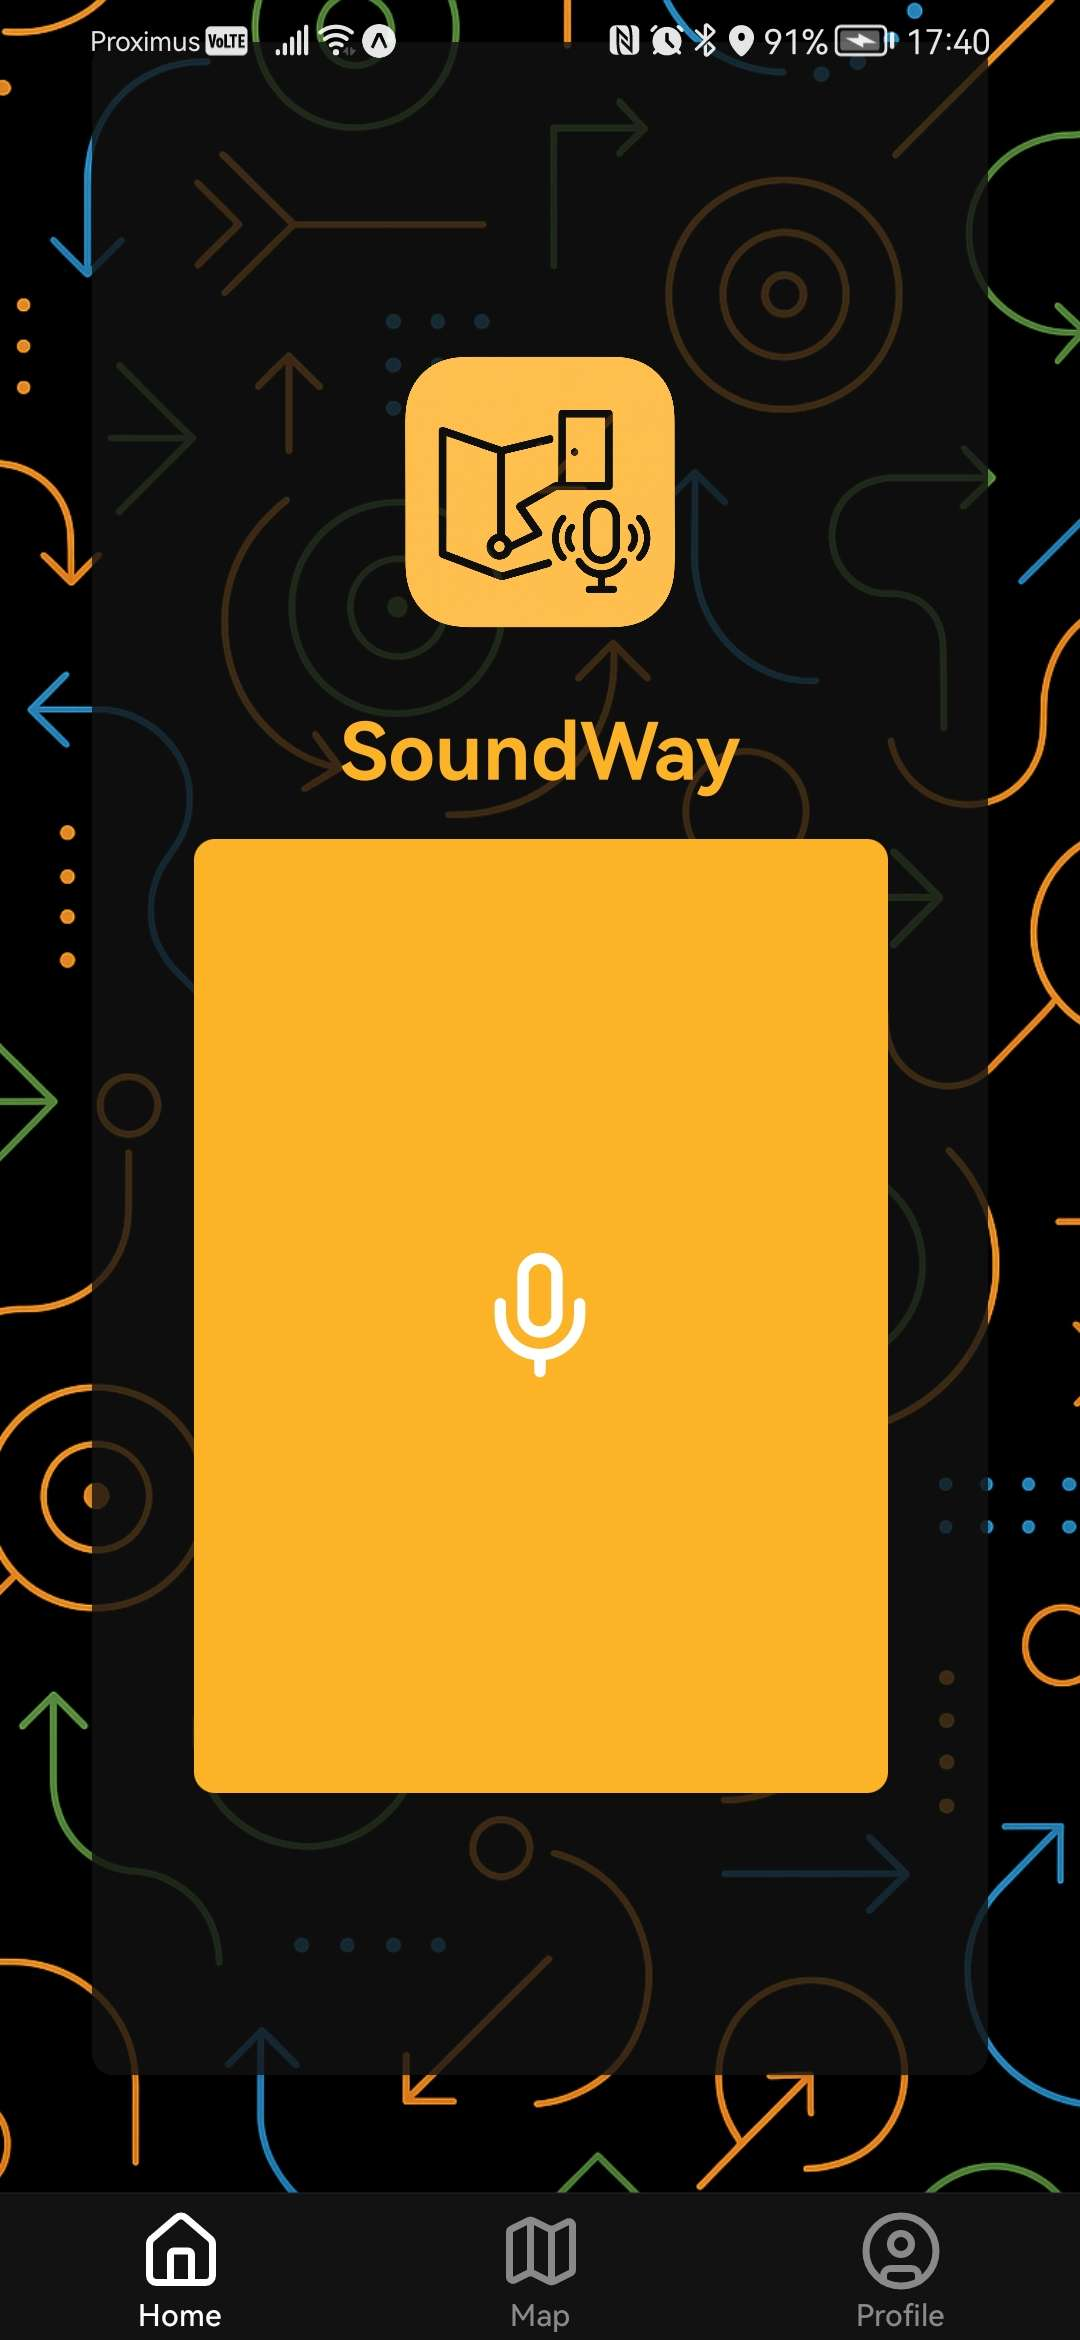
\includegraphics[width=\linewidth]{figures/soundway-voice.jpg}
    \end{minipage}\hfill
    \begin{minipage}{0.25\linewidth}
        \centering
        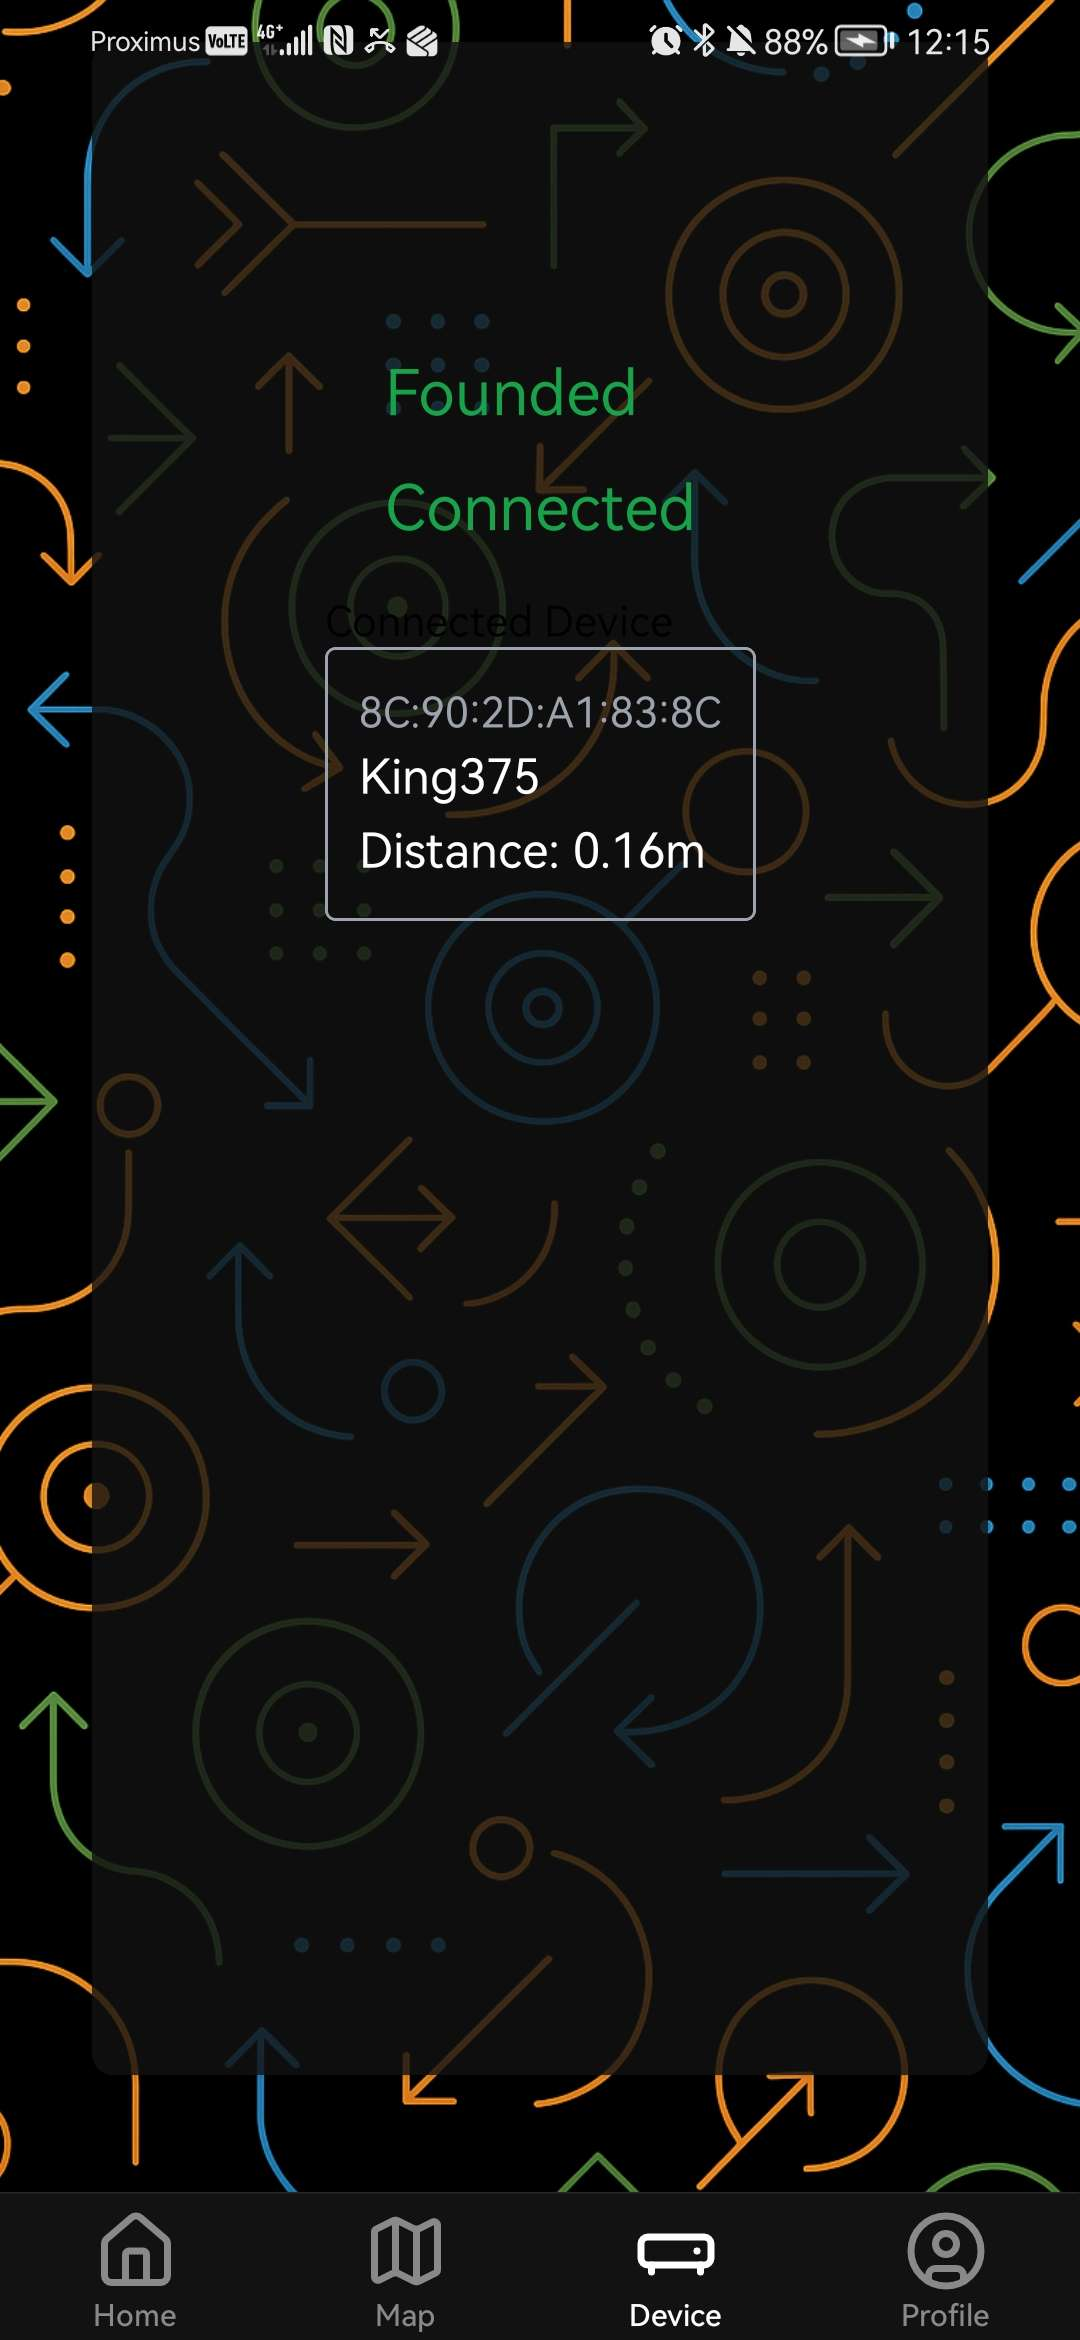
\includegraphics[width=\linewidth]{figures/soundway-distance.jpg}
    \end{minipage}
    \caption{Key screens of the SoundWay mobile application: login, voice interaction, and distance feedback.}
    \label{fig:app_screens}
\end{figure}

\section*{Appendix B: BLE Multi-Advertising Demonstration}

Figure~\ref{fig:ble_demo} illustrates the BLE scanning interface used during system testing. It shows the received RSSI values from the Raspberry Pi multi-advertising emitter (\texttt{King375}) and the signal variability observed in indoor corridors.

\begin{figure}[!htbp]
    \centering
    % photo à définir j'ai mis une autre en attendant
    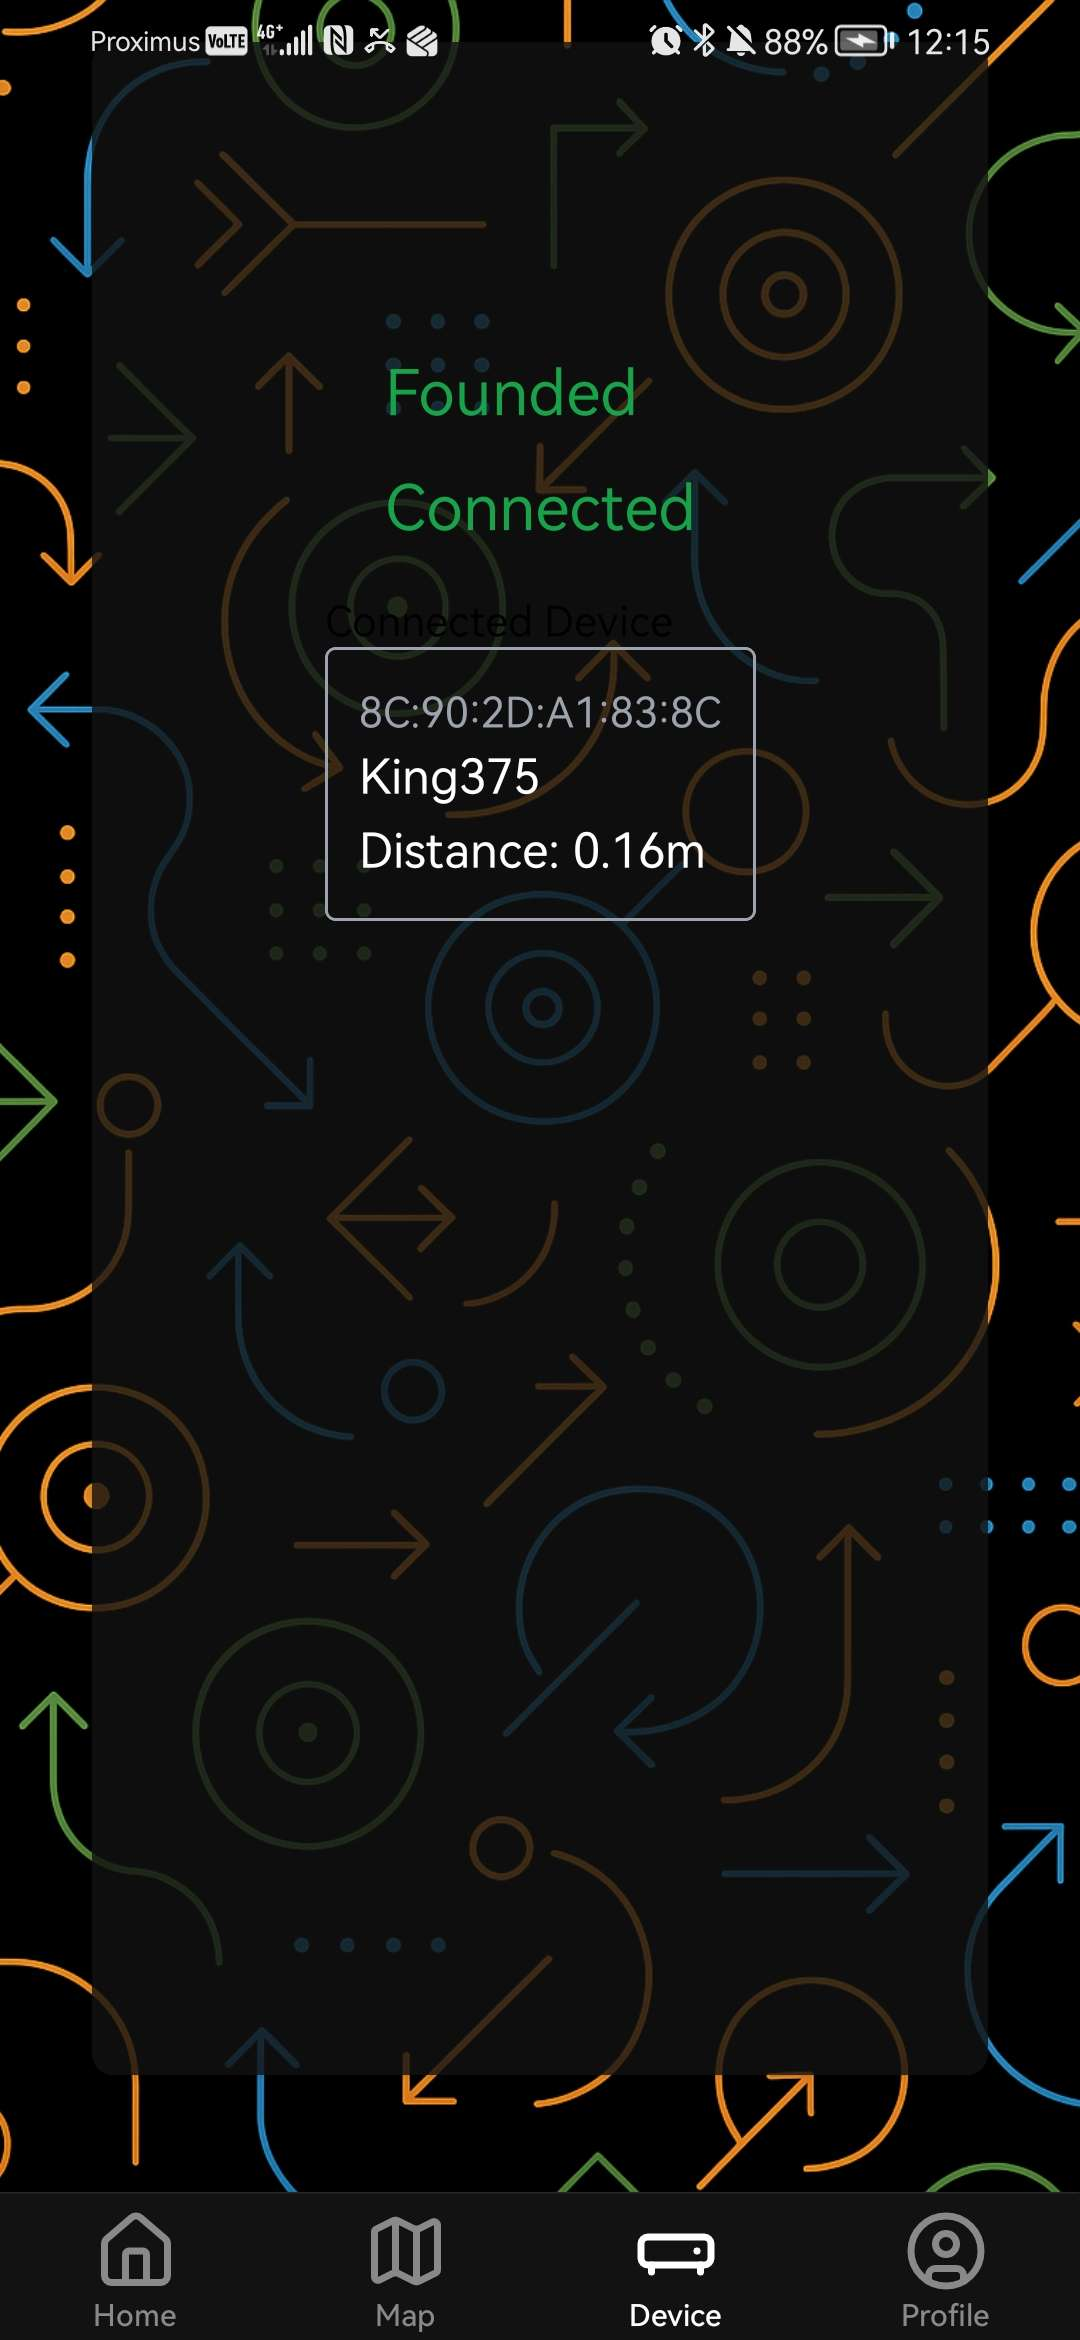
\includegraphics[width=0.2\linewidth]{figures/soundway-distance.jpg}
    \caption{BLE scanning interface showing the multi-advertising emission pattern and RSSI feedback.}
    \label{fig:ble_demo}
\end{figure}

Additional implementation details and source code excerpts are available in the online appendix.


\bibliographystyle{ACM-Reference-Format}
\bibliography{bibliography}

\end{document}
\endinput
